\section{Introduction}

Informal housing is a common issue faced by cities in developing countries. Inhabitants of informal regions, commonly known as slums, have less social economic opportunities and a lower quality of life compared to urban residents living in formal housing. Monitoring and controlling slum development requires resources that the government often cannot spare. Remote sensing methods from satellites provide a relatively low-cost solution in tracking the development of slums in the city. The detection of informal areas from the images provided by satellites remains a challenging task despite the effort from the field of study. This is in part caused by the disparate nature of slums, which varies between cities and even between regions of the same city. In this thesis, we aim to detect slums characterized by small buildings similar to tents with roofs often covered by blue plastic fabric. These properties indicate a newly developing slum, which often has a lack of basic services, such as infrastructure and sanitation. Over time, the inhabitants of these slums improve the build quality of the slums, converting them into permanent housing. Slum upgrading efforts by the government and third parties aim to support these slums by providing essential services to these newly developed neighborhoods.

%TODO: write about general thesis goal
% This thesis aims to detect the described slums from satellite images to provide governments with a low cost solution to obtain information about slum development. This enables these governments to support the needs of these developing neighborhoods.

\subsection{Global Context}
% state
According to Un-Habitat, close to a third of the global urban population lives in informal settlements \cite{2016state}. In specific parts of the world, for instance, Sub-Saharan Africa, the urban population that lives in informal housing is estimated to be close to two-thirds of the total urban population \cite{un2013planning}. In the past decades, the percentage of slum inhabitants compared to the urban population has decreased. Paradoxically, the absolute number of inhabitants since increased\cite{2016state}.

% definition and negative effects
Informal settlements exist globally, although they often occur in different forms and are described under different names. The individuals living in slums are specified by Un-Habitat as experiencing one or more of the following conditions: inadequate drinking water, inadequate sanitation, poor  structural quality of housing, overcrowding, and insecurity of tenure \cite{un2015slum}. In addition, the inhabitants of slums experience social and economic exclusion from the opportunities that an urban environment offers. Moreover, slum dwellers have an increased risk to suffer natural disasters and diseases. 

% solution
Over the years, there have been multiple governmental policies implemented to address the problem of informal settlements, which were initially primarily tolerated and neglected after large eviction and resettlement of the inhabitants were not found to be effective \cite{kuffer2016slums}. Instead, in recent years, slum upgrading is often used as a solution to the slum problem. This method enables governments to remove the adverse effects of slums by supporting the upgrade to formal housing \cite{cobbett2013cities}. Besides governments, Un-Habitat itself promotes and implements this method itself\cite{2015globact}.

\subsection{Related works and contributions}
% into remote sensing
In many cities in the developing world, slums are a large part of the urban environment. However, there is often a lack of information about the properties of the slums, such as the location, scale, and population \cite{kuffer2016slums}. These cities often do not have the resources to obtain this information through ground-survey. This is in part caused by the dynamic nature of slums, which causes ground surveys to get obsolete in only a short time. Slum detection using remote sensing can offer relatively low-cost up-to-date overviews of the slums in the city.

% methods
In the last decade, access to satellite images was becoming widespread, which coincided with an increase in methods for urban area classification \cite{kuffer2016slums}. This allowed for informal areas to be studied throughout the globe, e.g. Colombo \cite{colombo}, Johannesburg \cite{williams2016automatic}, Accra \cite{accra}, Mumbai \cite{mumbai}, Rio de Janeiro \cite{hofmann2008detecting}, and Hyderabad \cite{hyderabad}. With the increasing interest in slum detection, it became apparent that the structural characteristics of slums were quite different from formal areas, resulting in a large number of approaches based on the extraction of image-based features from satellite images. These approaches are, among others: the presence of vegetation \cite{niebergall2007object}, the size and shapes of buildings \cite{hofmann2008detecting}, the roofing material \cite{williams2016automatic}, texture features \cite{mattia2007exploiting}, and road accessibility \cite{owen2013approach}.

Currently, the majority of studies uses the pixel image data of informal regions to extract features \cite{kuffer2016slums}. A different approach would be the characterization of areas by the objects that inhabit them, for example, the detection of individual roofs in a certain area of an image \cite{williams2016automatic}. Another example of this object-based approach is the detection of road systems to characterize image regions. Alternatively, studies have used land use information \cite{novack2010urban} or social economical statistics \cite{engstrom2011using} to detect informal settlements.

% results
% The performance of the methods used in the studies is very variable. There are studies that have achieved a very high accuracy of in the 90\%. 

% conclusion prev work
%Because slums vary incredibly between different cities and regions, it is hard to obtain consensus about characteristics that well define informal areas. This variety makes it hard to create a method that will capture all the types of informal areas. As a result, the results obtained by the studies are quite specific to the studied city or area. 

 
\subsection{Proposed Method}

Our thesis continues with the work performed by Graesser \textit{et al.} \cite{graesser2012image}. The paper characterized formal and informal neighborhoods using a set of different features extracted from satellite images. Their approach was able to successfully characterize the two types of neighborhoods with high accuracy in certain parts of the urban landscape. We will evaluate two of the feature extraction methods described in the paper from Graesser \textit{et al.} and attempt to reproduce similar results with satellite images from Bangalore. These methods are the Histogram of Oriented Gradients and Line support regions. Beyond the replication and evaluation of previous research, the methods of feature extraction used by Graesser \textit{et al.} are extended with an additional new method. This method creates a feature based on the density of road intersections in an image. The feature created from this method will be compared to the existing features and measured for its performance. The features produced by the three methods will combined and used by a set of different classification methods. We will evaluate the different classification methods to discover the most suitable classification method for our image and its features. 



\subsection{Data and Area of Study}
The image data used for the thesis is displayed in Figure \ref{fig:sections}d, a larger version of the image is included in appendix A. The content of this image contain a large area of Bangalore, which is the capital city of the Indian state of Karnataka, located in south-central India. Bangalore experienced fast growth in population from 8.4 million in 2011 to 12.3 million in 2017, becoming the third largest city in India\cite{popcount2017}. One of the reasons for its sudden growth is the large IT sector together with better living standards and infrastructure. This rapid increase in population has led to a shortage of housing which, in turn, caused an increase in the number of slums in the city. At present, the city is estimated to have over two thousand slums. These slums account for 25 to 35 percent of the urban population \cite{roy2018survey}.

The image in Figure \ref{fig:sections}d has a resolution of 52,322 by 31,789 pixels with a file size of 6.19GiB and extends in latitude and longitude from  (12\degree54'22.729", 77\degree31'58.631") in the south-west to (12\degree59'37.414", 77\degree40'37.776") in the northeast. The image was created in 2016 by the earth observation satellite WorldView3 owned by DigitalGlobe. The WorldView3 satellite produces multiple types of images with varying degrees of resolution. The panchromatic images have a resolution of 0.31 meter in contrast to the multiband images have a significantly lower resolution of 1.24 meter. The project uses pan-sharpened images, which combines the high resolution panchromatic- and the low-resolution multiband images to create high-resolution RGB images.

% Source of shape files
Besides image data, we also use shapefiles with the vectorized location and shape of the slums in Bangalore. This data is gathered in the field by a third party using GPS tracking in June of 2016. These shapes files are displayed on top of the satellite images in Figure \ref{fig:sections} and mark the location of the slums. The images a to c show that these slums are relatively small in scale compared to the surrounding neighborhoods. These sections show the dispersed small blue roofs that characterize the slums in Bangalore. 

\subsection{Challenges}

The distinction between formal and informal regions is often quite challenging. There are a lot of factors that could introduce noise to the dataset, hindering correct classification. For instance, some areas might have been missed during the survey. Also, the shapefile defining boundaries of the slums are simplified in shape and sometimes imprecise in location as well. The location of the slums and the shapes of the boundaries can be observed in Figure \ref{fig:sections}. As a result of these sharp and simple shapes,  areas that are not part of a slum by itself are included as slums nevertheless, for example, parts of roads, vegetation or open spaces. Moreover, the shapefile was not created at the same time as the satellite image; the shapefiles were created a few months after the satellite image was captured. This is especially a problem since the slums in Bangalore are very dynamic and can change drastically in just a few months. It is therefore important to use shapefiles and satellite images from similar dates. A difference between the shapefile and the satellite image will very likely increase the number of false positives and negatives. An example of the difference between shapefile and satellite image can be seen in Figure \ref{fig:sections} b. In the middle left of Section 2, there is a large patch of blue roofs that is very likely a slum even though it is not annotated as such. Similar discrepancies occur in the other sections as well. 

% TODO: appendix -v
Besides noise in the dataset, another challenge is the scarcity of informal settlements.  The slums we aim to detect are small and highly distributed throughout the city. Figure \ref{fig:sections}d illustrates this point quite well. The relatively small number of slums causes the dataset of formal and informal regions to become quite skewed.

In our case, everything that is not the specific type of slum we are looking for is automatically considered formal, which actually often not true. Instead of formal housing, this class includes a large range of different types of buildings. Furthermore, fields and lakes in the image are also included in the formal class. Therefore, the formal class should be considered as the class that includes all things except a specific type of slum. As a result, the formal regions will have a large amount of variance of visual properties in the image. The diverse content of the formal class of visual characteristics might hinder the effectiveness of classification between formal and informal regions. However, this is the only class division that is possible since we do not possess the location and shapes of the other types of land cover.

The satellite image displayed in Figure \ref{fig:sections}d is transformed into the three smaller sections, displayed in Figure \ref{fig:sections} a to c, to reduce the skewness between the two classes. These sections are selected on the relative prevalence of informal settlements in that specific part of the image. The location of the sections relative to the complete image is displayed in Figure \ref{fig:sections}d as red squares. The use of these sections should provide a less one-sided class balance and consequently increase classification performance. 

%\begin{figure}
%\centering
%  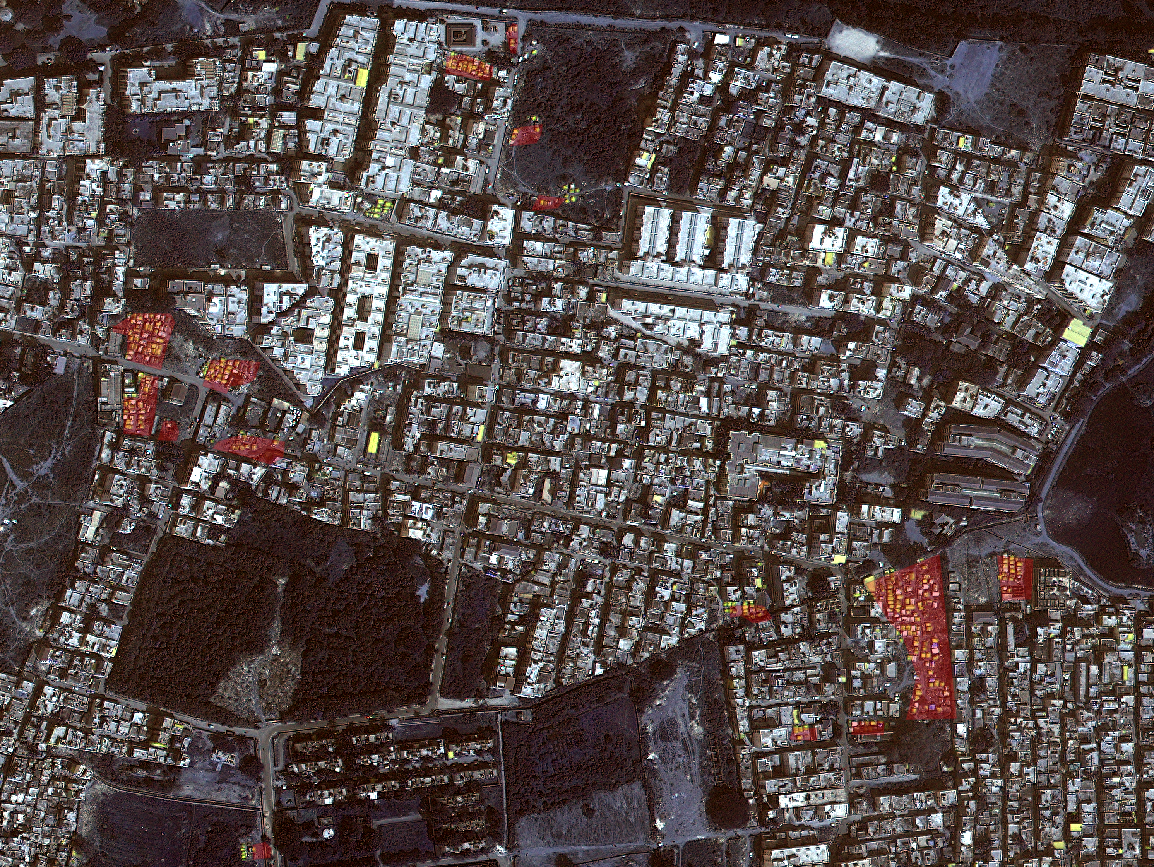
\includegraphics[width=\linewidth]{images/section_3}
%  \caption{Dense informal area in Bangalore, the red patches indicate informal
%  settlements}
%  \label{fig:section_3}
%\end{figure}

\begin{figure}
\centering
\begin{tabular}{cc}
  \subfloat[Section 1]{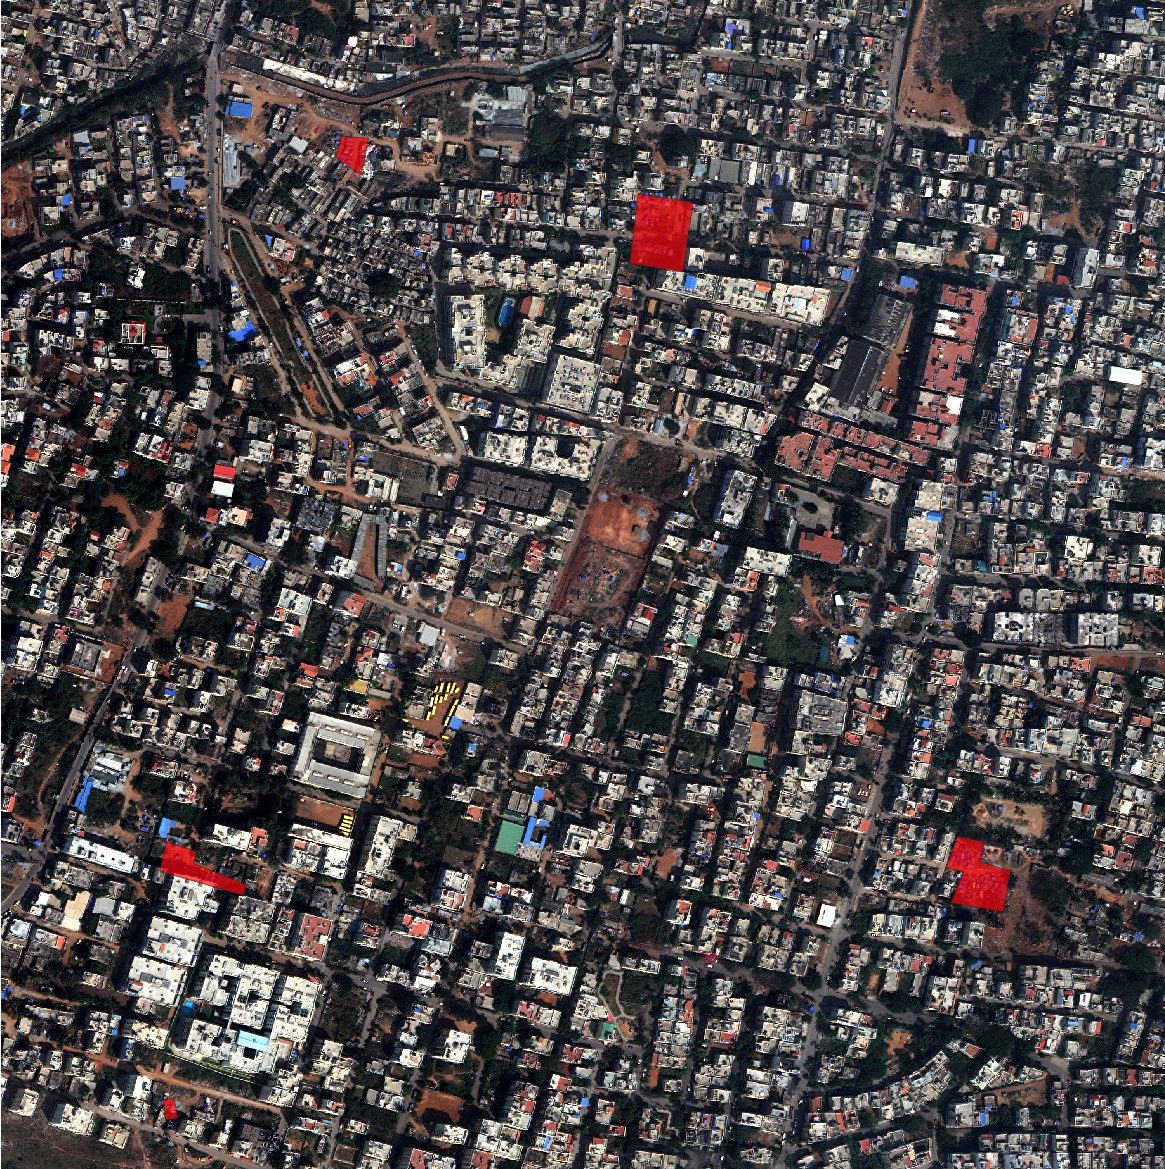
\includegraphics[width=.5\textwidth, height=.5\textwidth]{images/section_1_gt}}&
  \subfloat[Section 2]{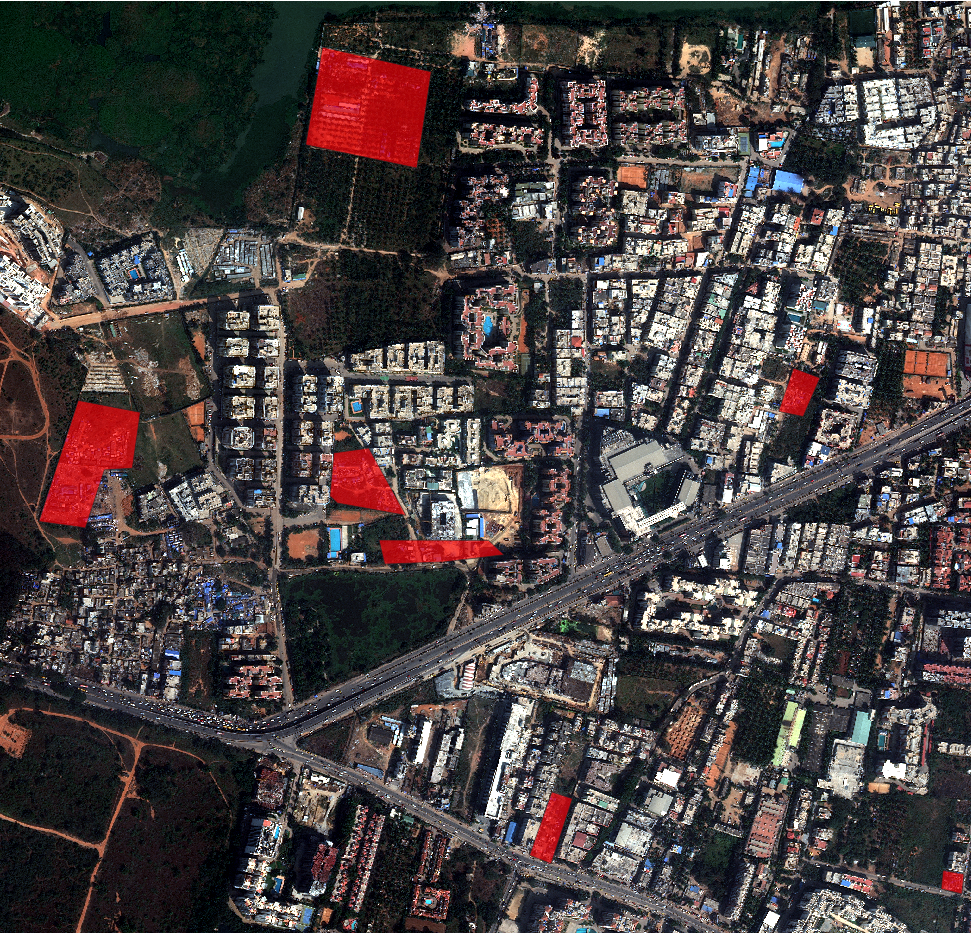
\includegraphics[width=.5\textwidth, height=.5\textwidth]{images/section_2_gt}}\\
  \subfloat[Section 3]{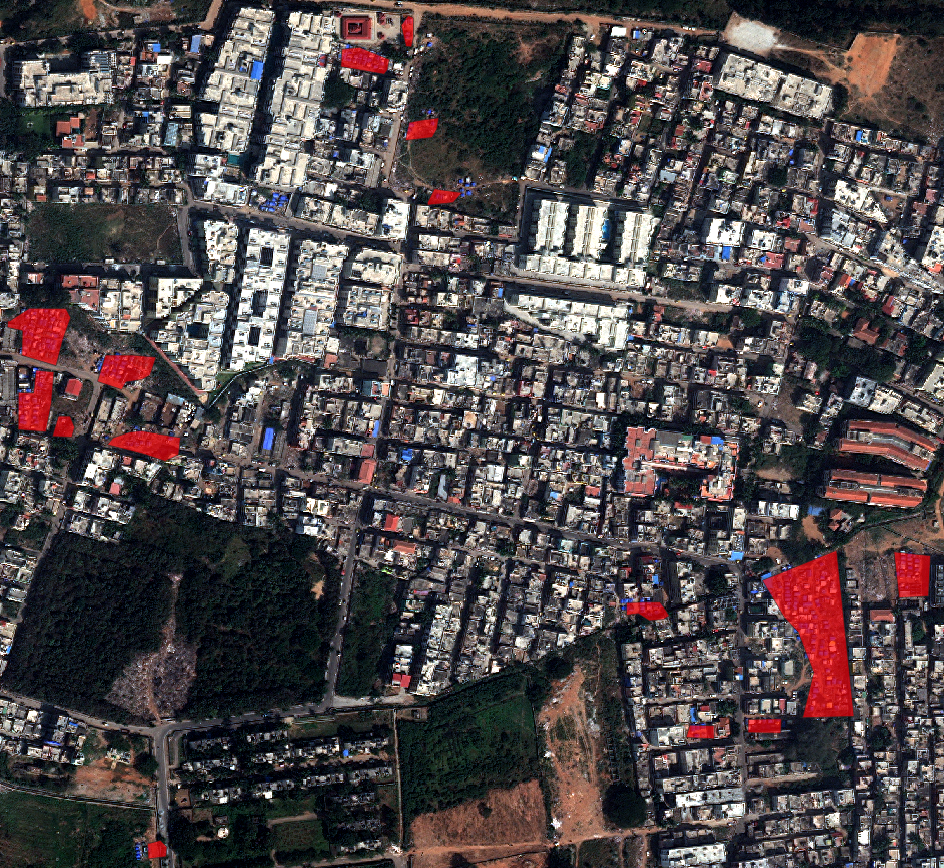
\includegraphics[width=.5\textwidth, height=.5\textwidth]{images/section_3_gt}}&
  \subfloat[Location of Sections]{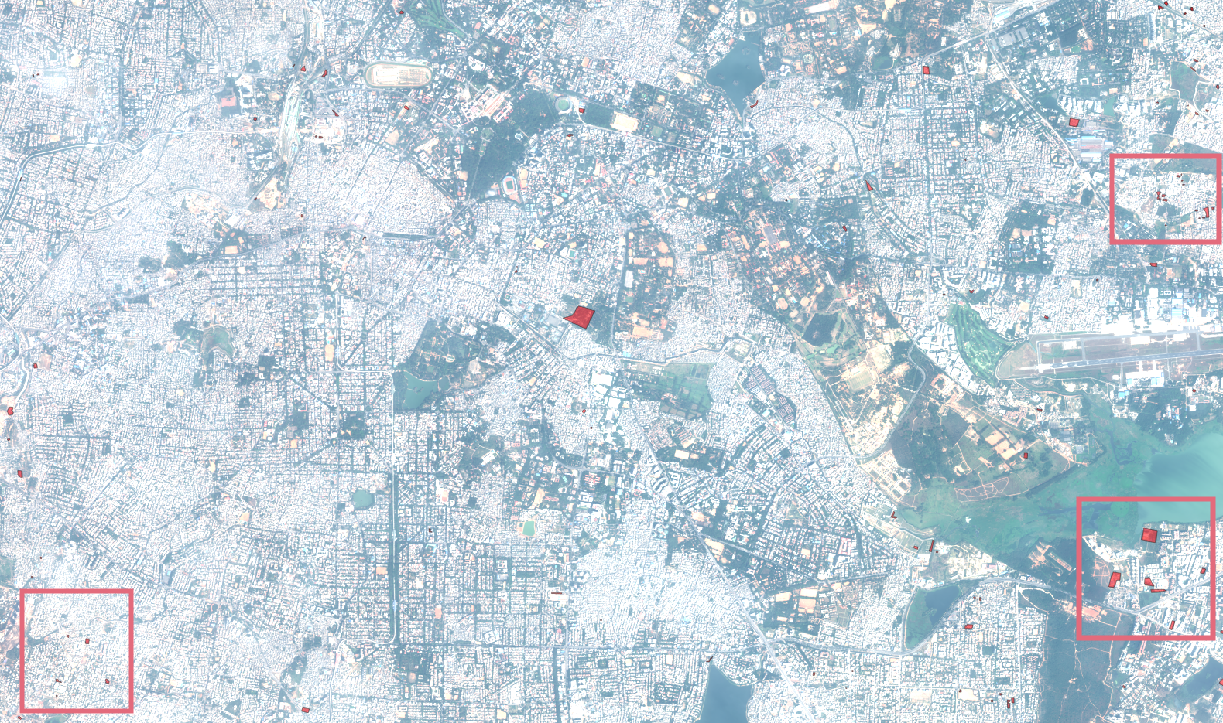
\includegraphics[width=.5\textwidth]{images/west-bangalore_sections}}
\end{tabular}
\caption{The images used for evaluation and classification}
\label{fig:sections}
\end{figure}

